\documentclass[justified]{tufte-handout}
\usepackage{braph2_tut}
%\geometry{showframe} % display margins for debugging page layout

\title{Brain Atlas}

\author[The BRAPH~2 Developers]{The BRAPH~2 Developers}

\begin{document}

\maketitle
	
\fig{marginfigure}
	{fig:01}
	{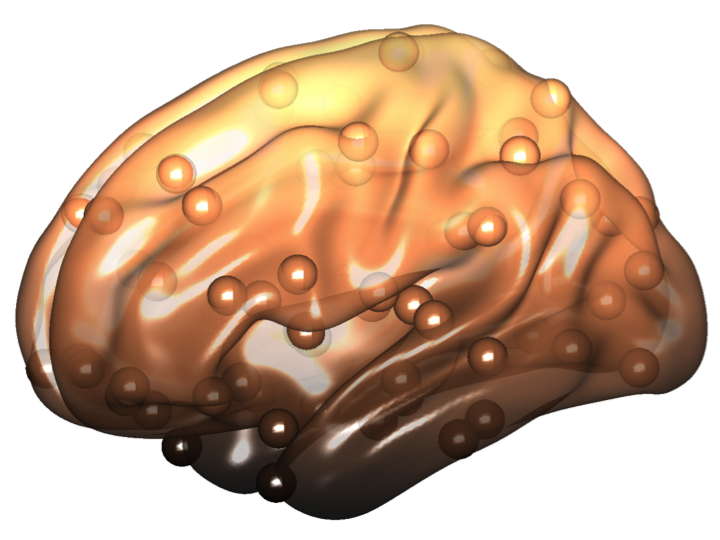
\includegraphics{tut_ba/fig0.png}}
	{Brain regions.}
	{
	Example of a brain surface image with some brain regions generated with BRAPH 2.0.
	}

\begin{abstract}
\noindent
This Tutorial explains how to work with the Graphical User Interface (GUI) to manage brain atlases.
This is typically the first step required to perform a graph analysis in BRAPH 2.0. 
In this Tutorial, we will explain you how to upload a brain atlas and how to visualize it.
\end{abstract}

\tableofcontents

\fig{figure*}
	{fig:02}
	{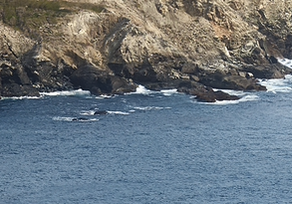
\includegraphics[height=10cm]{tut_ba/fig1.png}}
	{Brain Atlas GUI.}
	{
	Full graphical user interface to work with a brain atlas. 
	}

\clearpage
\section{Open the GUI}

The brain atlas GUI is typically the first step in the BRAPH 2.0 pipelines. You can also do it by typing braph2, which will open the Graphical User Interface of the BRAPH 2.0 software, which allows you to select a pipeline containing thesteps that you want to apply in your analysis. Once a pipeline has been selected, the first window will allow you to upload the brain atlas, as shown in \Figref{fig3}a.

\fig{figure*}
	{fig:02}
	{
	[h!]
	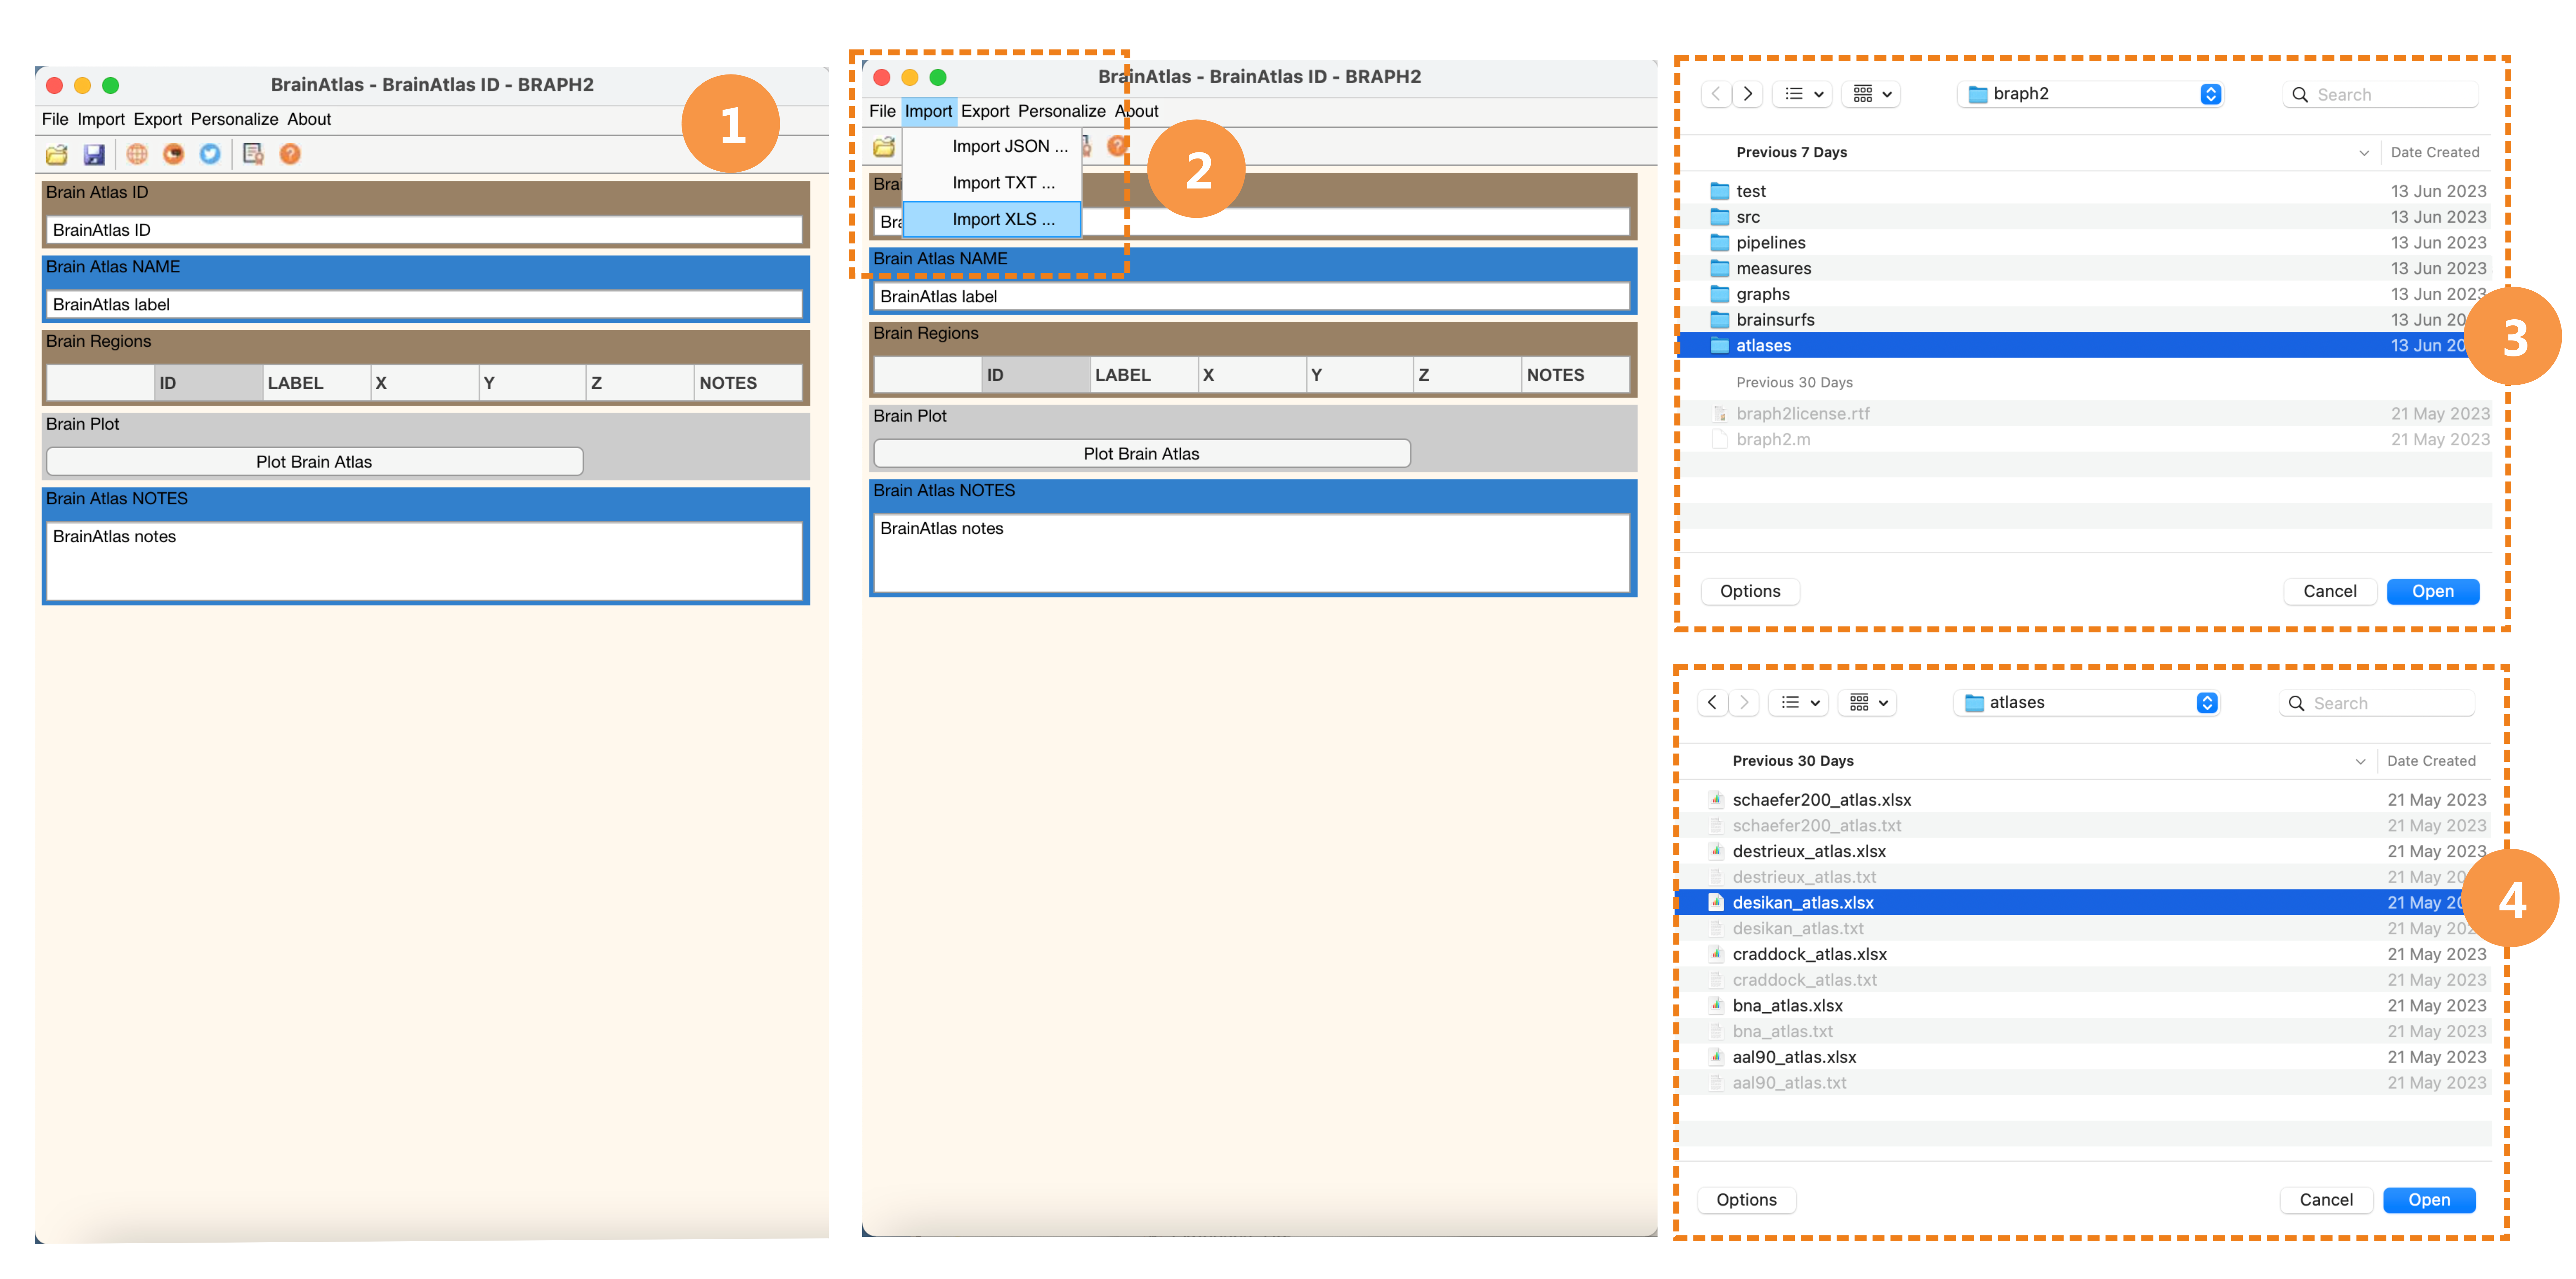
\includegraphics[height=10cm]{tut_ba/fig3.png}
	}
	{Brain Atlas GUI}
	{
	Uploading a brain atlas. 
	}

To open the GUI and upload the brain atlas, you can also do it from the command line by typing the commands in \Coderef{cd:launch}.
%
\begin{lstlisting}[
	label=cd:launch,
	caption={
		{\bf Code to launch the Brain Atlas GUI.}
		This code can be used in the MatLab command line to launch the  Brain Atlas GUI.
	}
]
ba = BrainAtlas(); ¥\circled{1}\circlednote{1}{creates a new object \code{BrainAtlas}.}¥

gui = GUIElement('PE', ba); ¥\circled{2}\circlednote{2}{creates a GUI to upload the brain atlas.}¥
gui.get('DRAW') ¥\circled{3}\circlednote{3}{draws the GUI.}¥
gui.get('SHOW') ¥\circled{4}\circlednote{4}{shows the GUI.}¥
\end{lstlisting}

\section{Upload the Brain Atlas}

In this window opened in the previous step (1) you have a menu that you can use to import a brain atlas (2) that you created or has already been prepared for you to use from the atlases folder of BRAPH 2.0 (3). In this example, we are uploading the Desikan atlas (4) \Figref{fig3} . 
	
\fig{figure*}
	{fig:xxx}
	{
	[h!]
	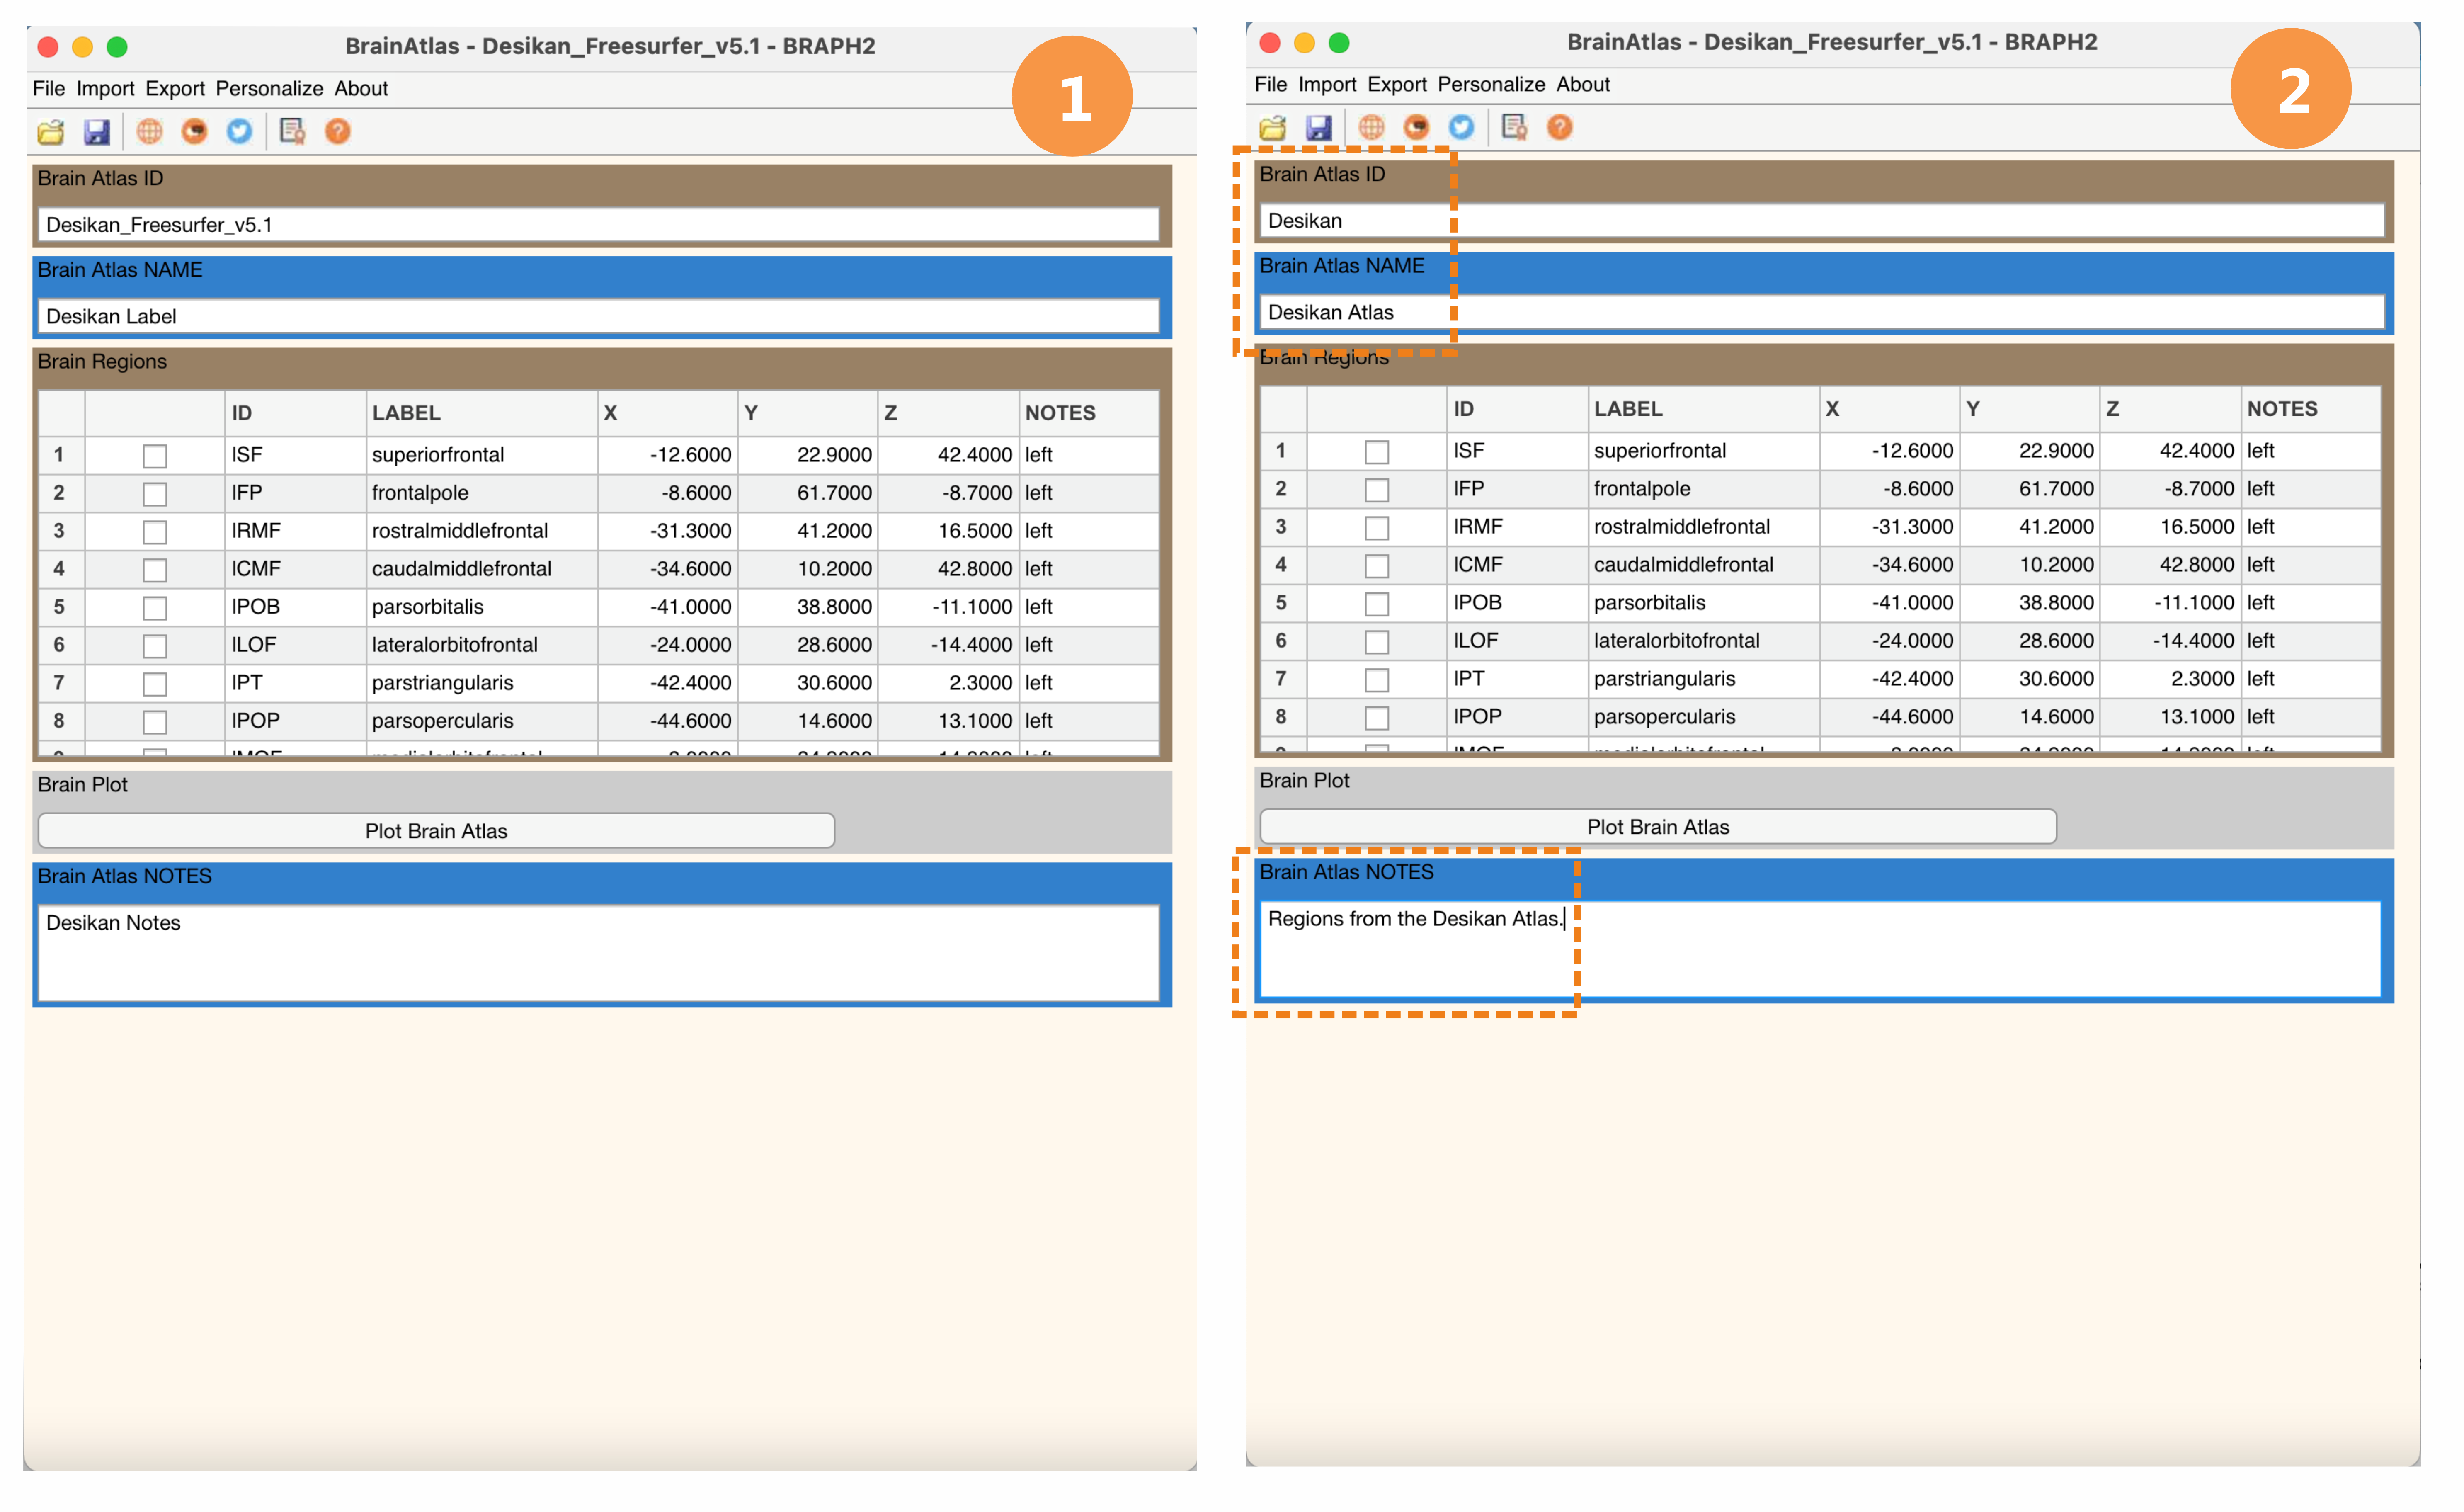
\includegraphics{tut_ba/fig4.png}
	}
	{Brain Atlas GUI.}
	{
	Changing information in the brain atlas GUI. 
	}

Note that you can change information in this GUI (1) such as the brain atlas ID, the brain atlas name, the brain atlas description (2) as well as the IDs, labels, coordinates and notes of the brain regions.

\clearpage
\section{Ready Brain Atlases}

\fig{figure}
	{fig:07}
	{
	[b!]
	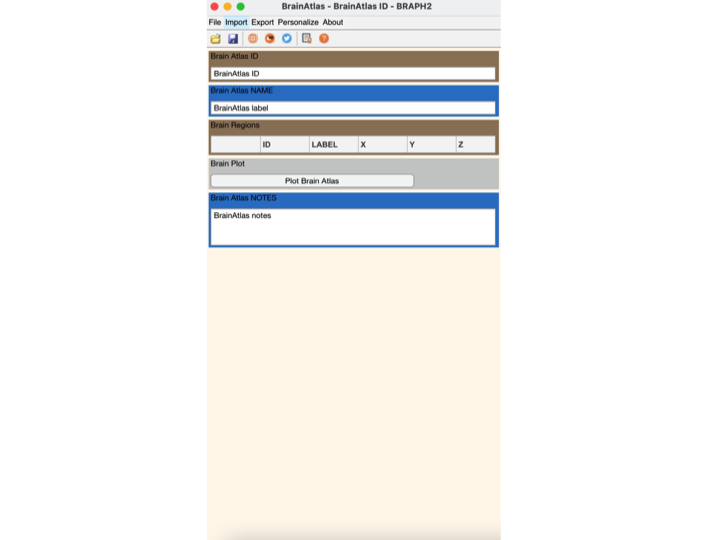
\includegraphics[height=15cm]{tut_ba/fig7.png}
	}
	{Brain Atlas GUI.}
	{
	Different brain atlases provided by BRAPH 2.0: \\
	{\bf AAL90} Automated Anatomical Labelling atlas with 90 cortical and subcortical regions.\\
	{\bf AAL116} Automated Anatomical Labelling atlas with 116 cortical and subcortical regions, including cerebellar areas.\\
	{\bf BNA} Brainnetome atlas with 246 cortical and subcortical regions.\\
	{\bf Craddock} Functional atlas with 200 cortical and subcortical regions.\\
	{\bf Desikan} Anatomical atlas with 68 cortical derived from the FreeSurfer software.\\
	{\bf Destrieux} Anatomical atlas with 148 cortical derived from the FreeSurfer software.\\
	{\bf Schaefer} Functional brain atlas with 200 cortical regions that belong to 7 different resting-state fMRI networks.
	}

Currently, we provide several brain atlases that are commonly used in the field of brain connectomics, which can be downloaded from our website (\url{http://braph.org/software/brain-atlases/}) \Figref{fig7}.

\clearpage
\section{Create a New Brain Atlas}

To prepare a Brain Atlas in BRAPH 2.0 format, you should create a new excel file (.xls or .xlsx), as shown in \Figref{fig2}. 

\fig{figure}
	{fig:02}
	{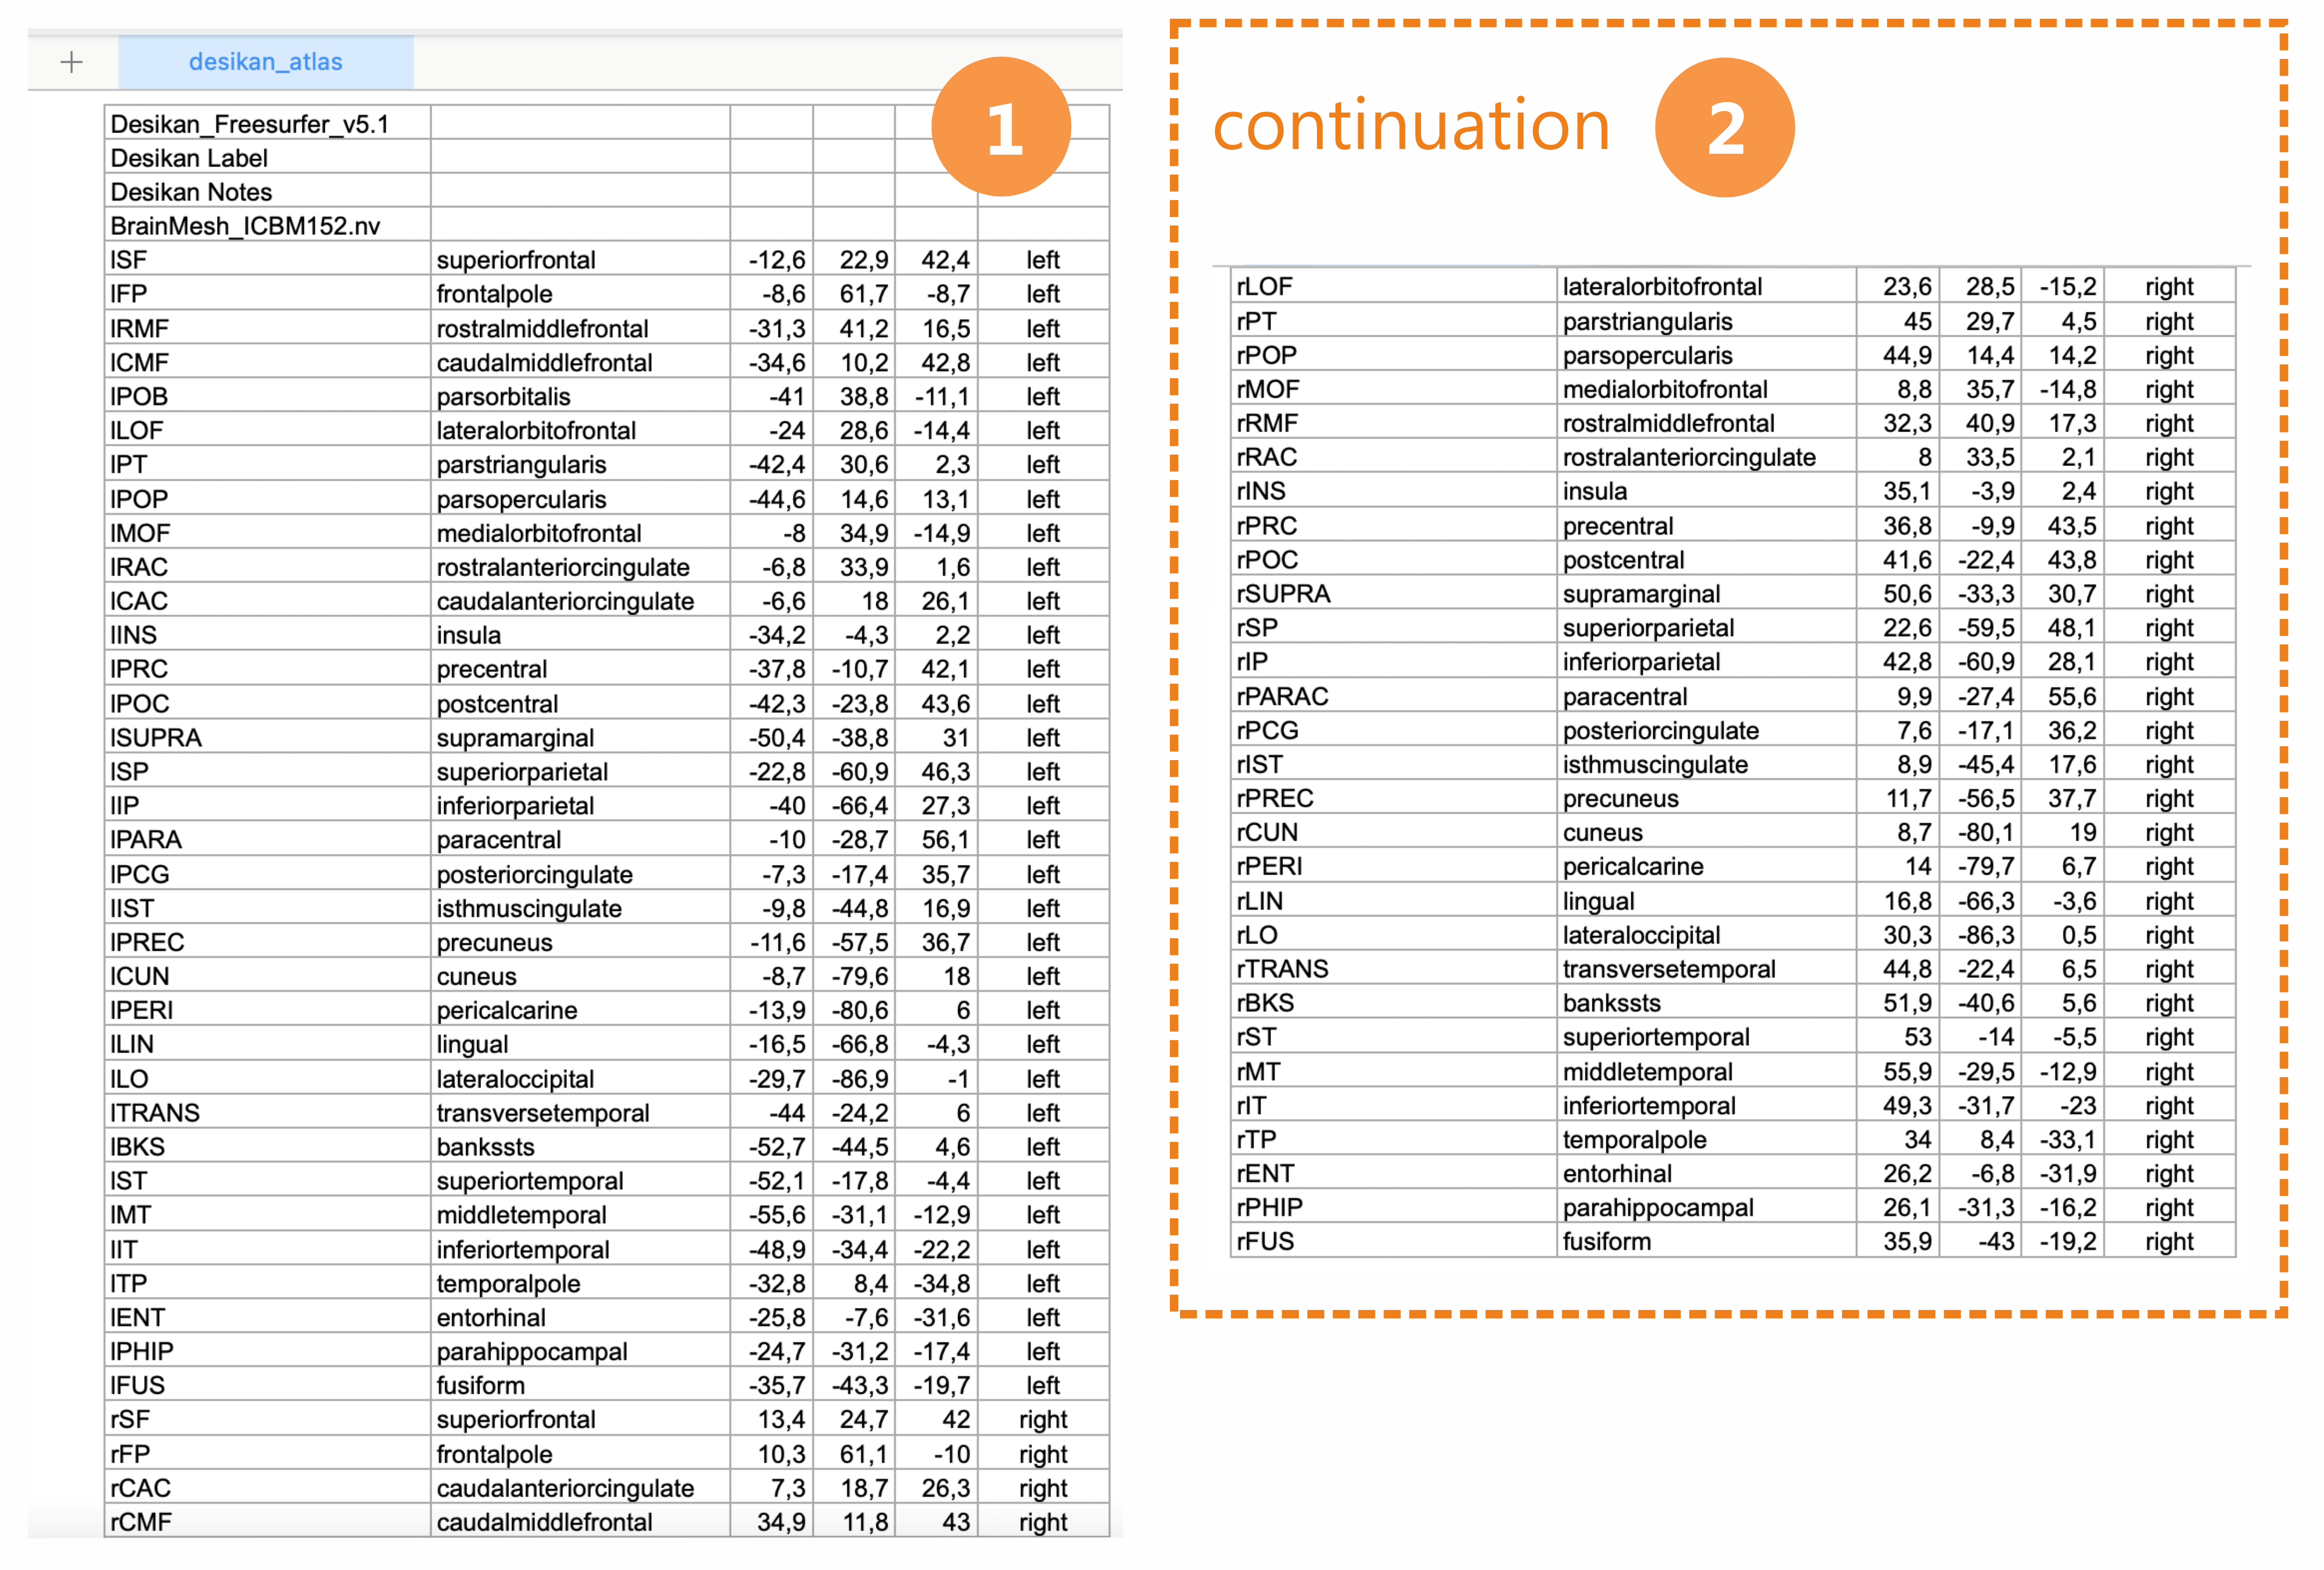
\includegraphics[height=10cm]{tut_ba/fig2.png}}
	{Brain Atlas GUI.}
	{
	Full graphical user interface to work with brain atlases. 
	}

Start by writing the following information in the first 4 rows:
\begin{itemize}

\item Brain Atlas ID (row 1, column 1). 
For example: Desikan FreeSurfer v5.1

\item Brain Atlas LABEL (row 2, column 1). 
For example: Desikan Labels

\item Brain Atlas NOTES (row 3, column 1).
For example: Desikan Nodes

\item Brain Surface Name (row 4, column 1).
For example: BrainMeshICBM152.nv

\end{itemize}
Then, from row 5, you should include the IDs of the regions of your atlas (1st column), the Labels of the regions of your atlas (2nd column), the X, Y and Z coordinates (3rd, 4th and 5th columns) and the brain hemisphere or any notes you would like to add (6th column).	

\clearpage
\section{Plot the Brain Atlas}

Once you are satisfied you can plot your brain atlas (1), which will open a brain surface that contains the nodes corresponding to brain regions (2) \Figref{fig5}.

\fig{figure*}
	{fig:05}
	{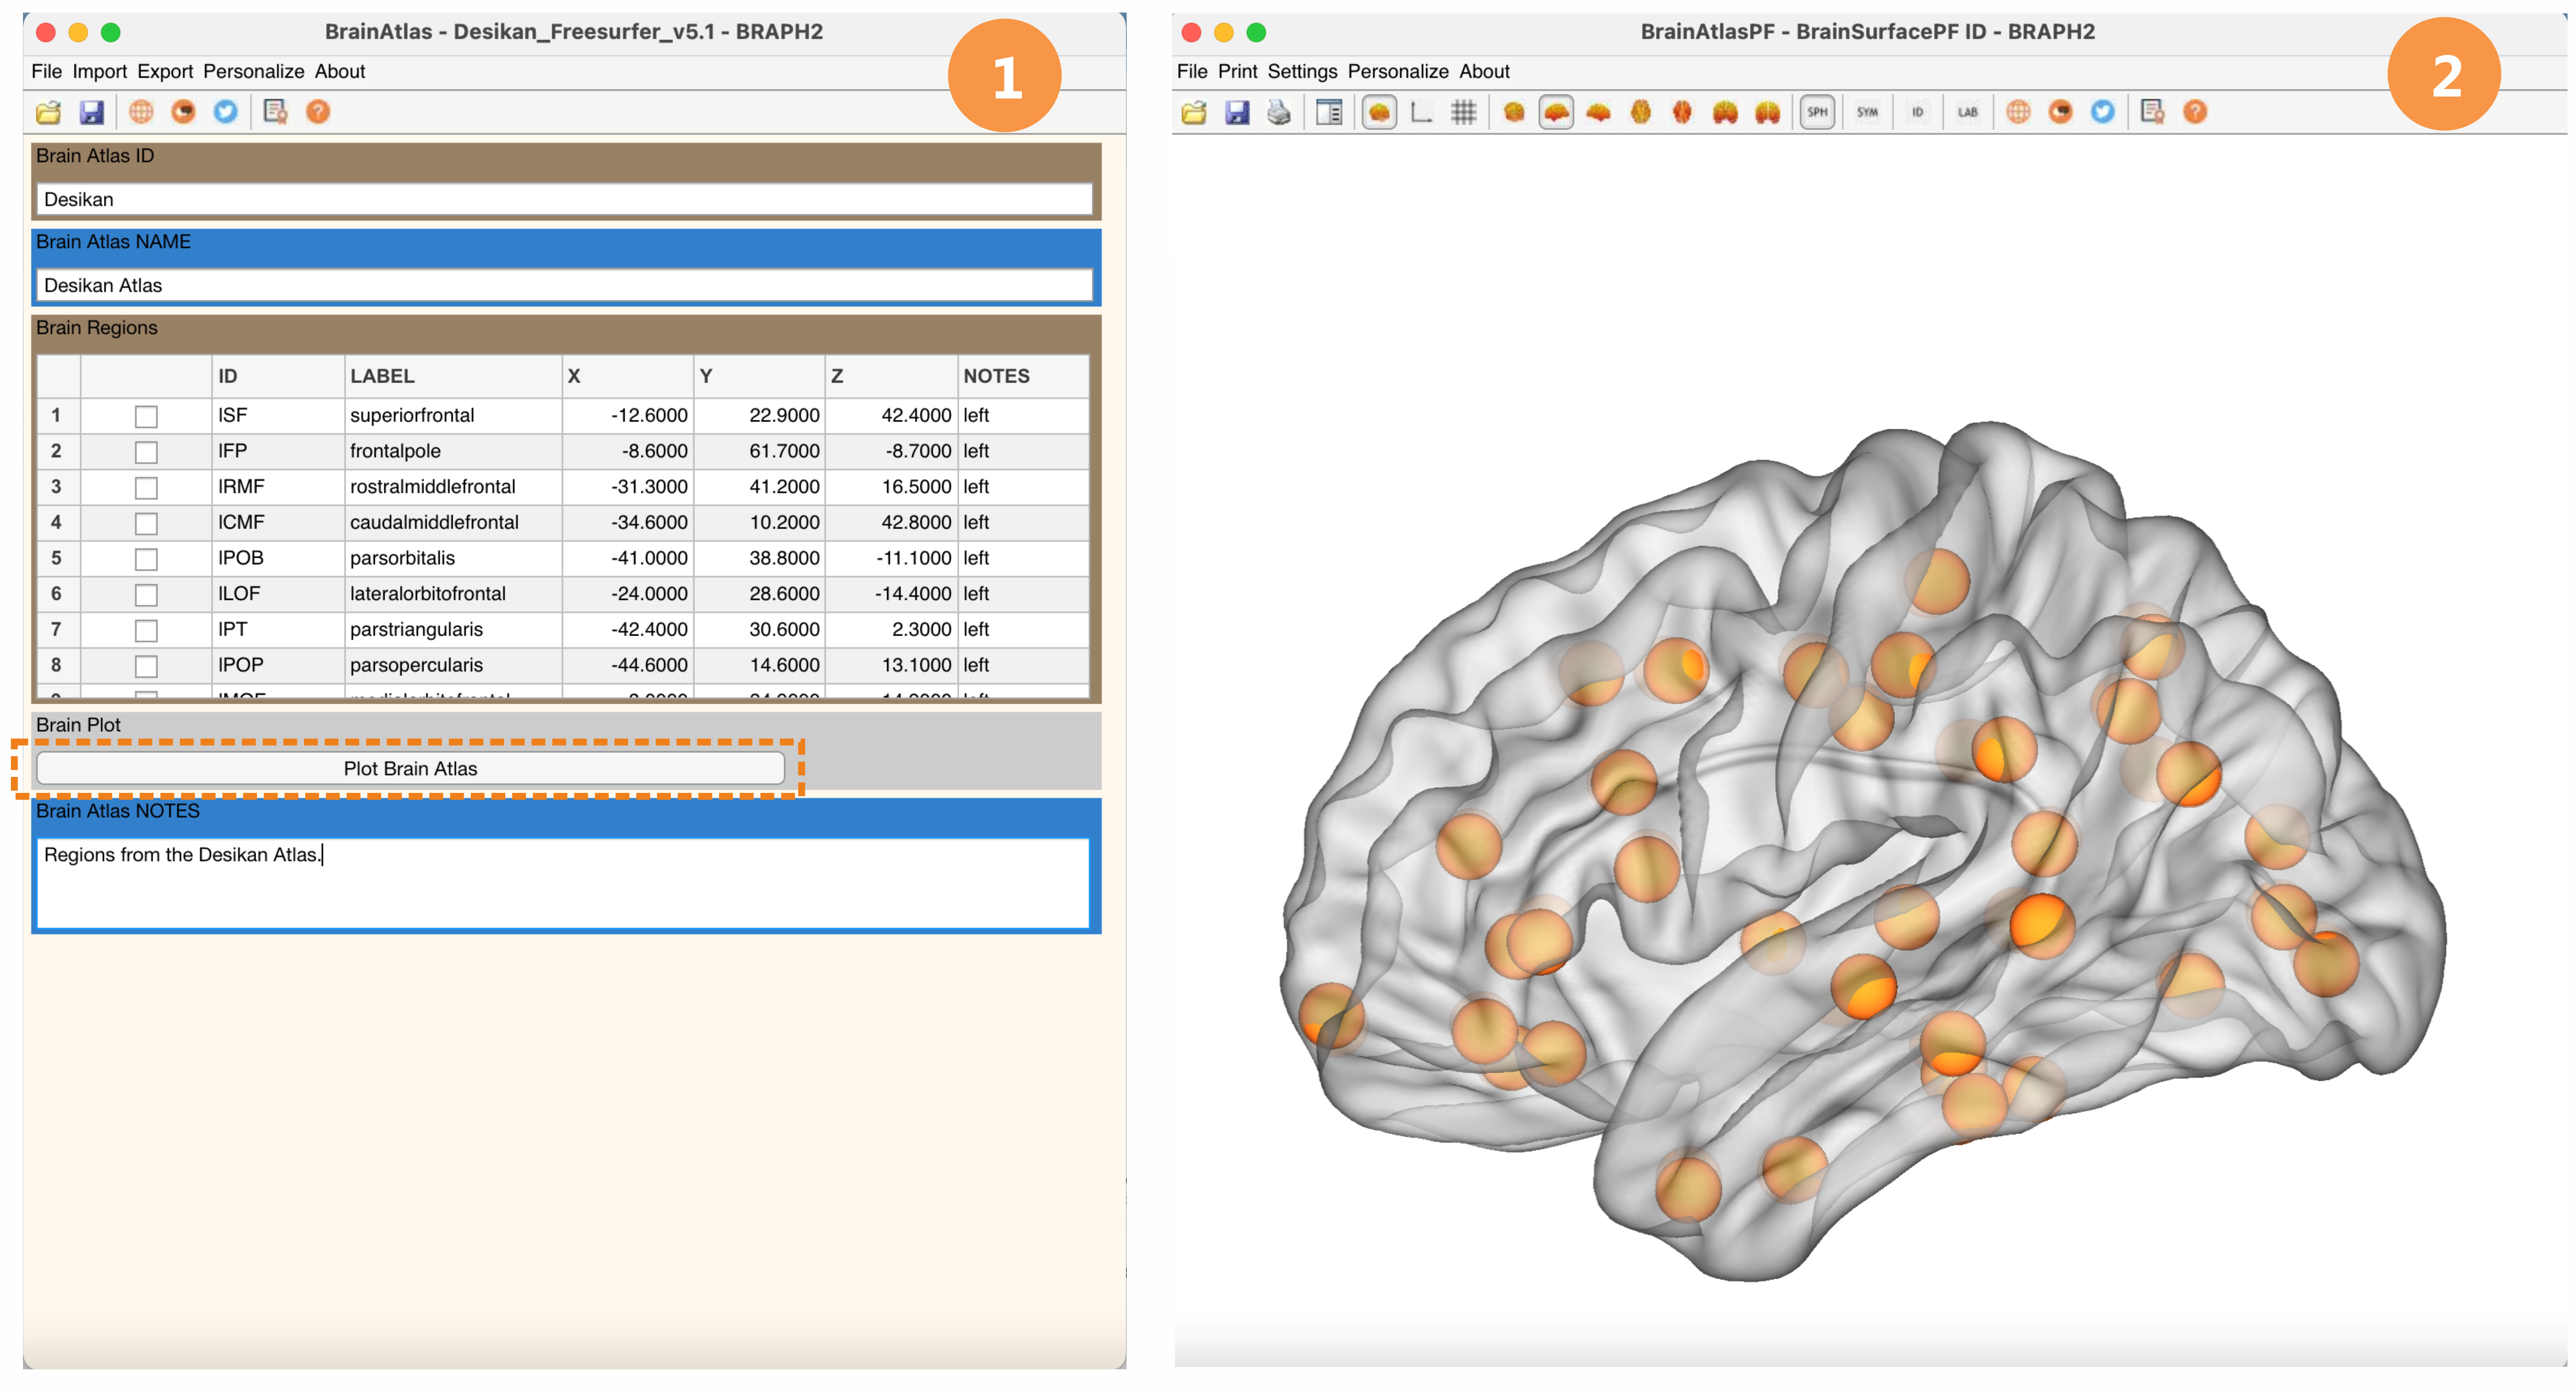
\includegraphics[height=10cm]{tut_ba/fig5.png}}
	{Brain Atlas GUI.}
	{
	Plotting the nodes of a brain atlas on a 3D brain surface. 
	}
	
This new window has a large menu that allows you to change the visualization of the atlas. We suggest you try the different options to understand how they change the figure. Importantly, within this menu there is one option called Settings Brain Surface (1) which, when selected, will open another window, as can be seen below \Figref{fig6}.

\fig{figure*}
	{fig:06}
	{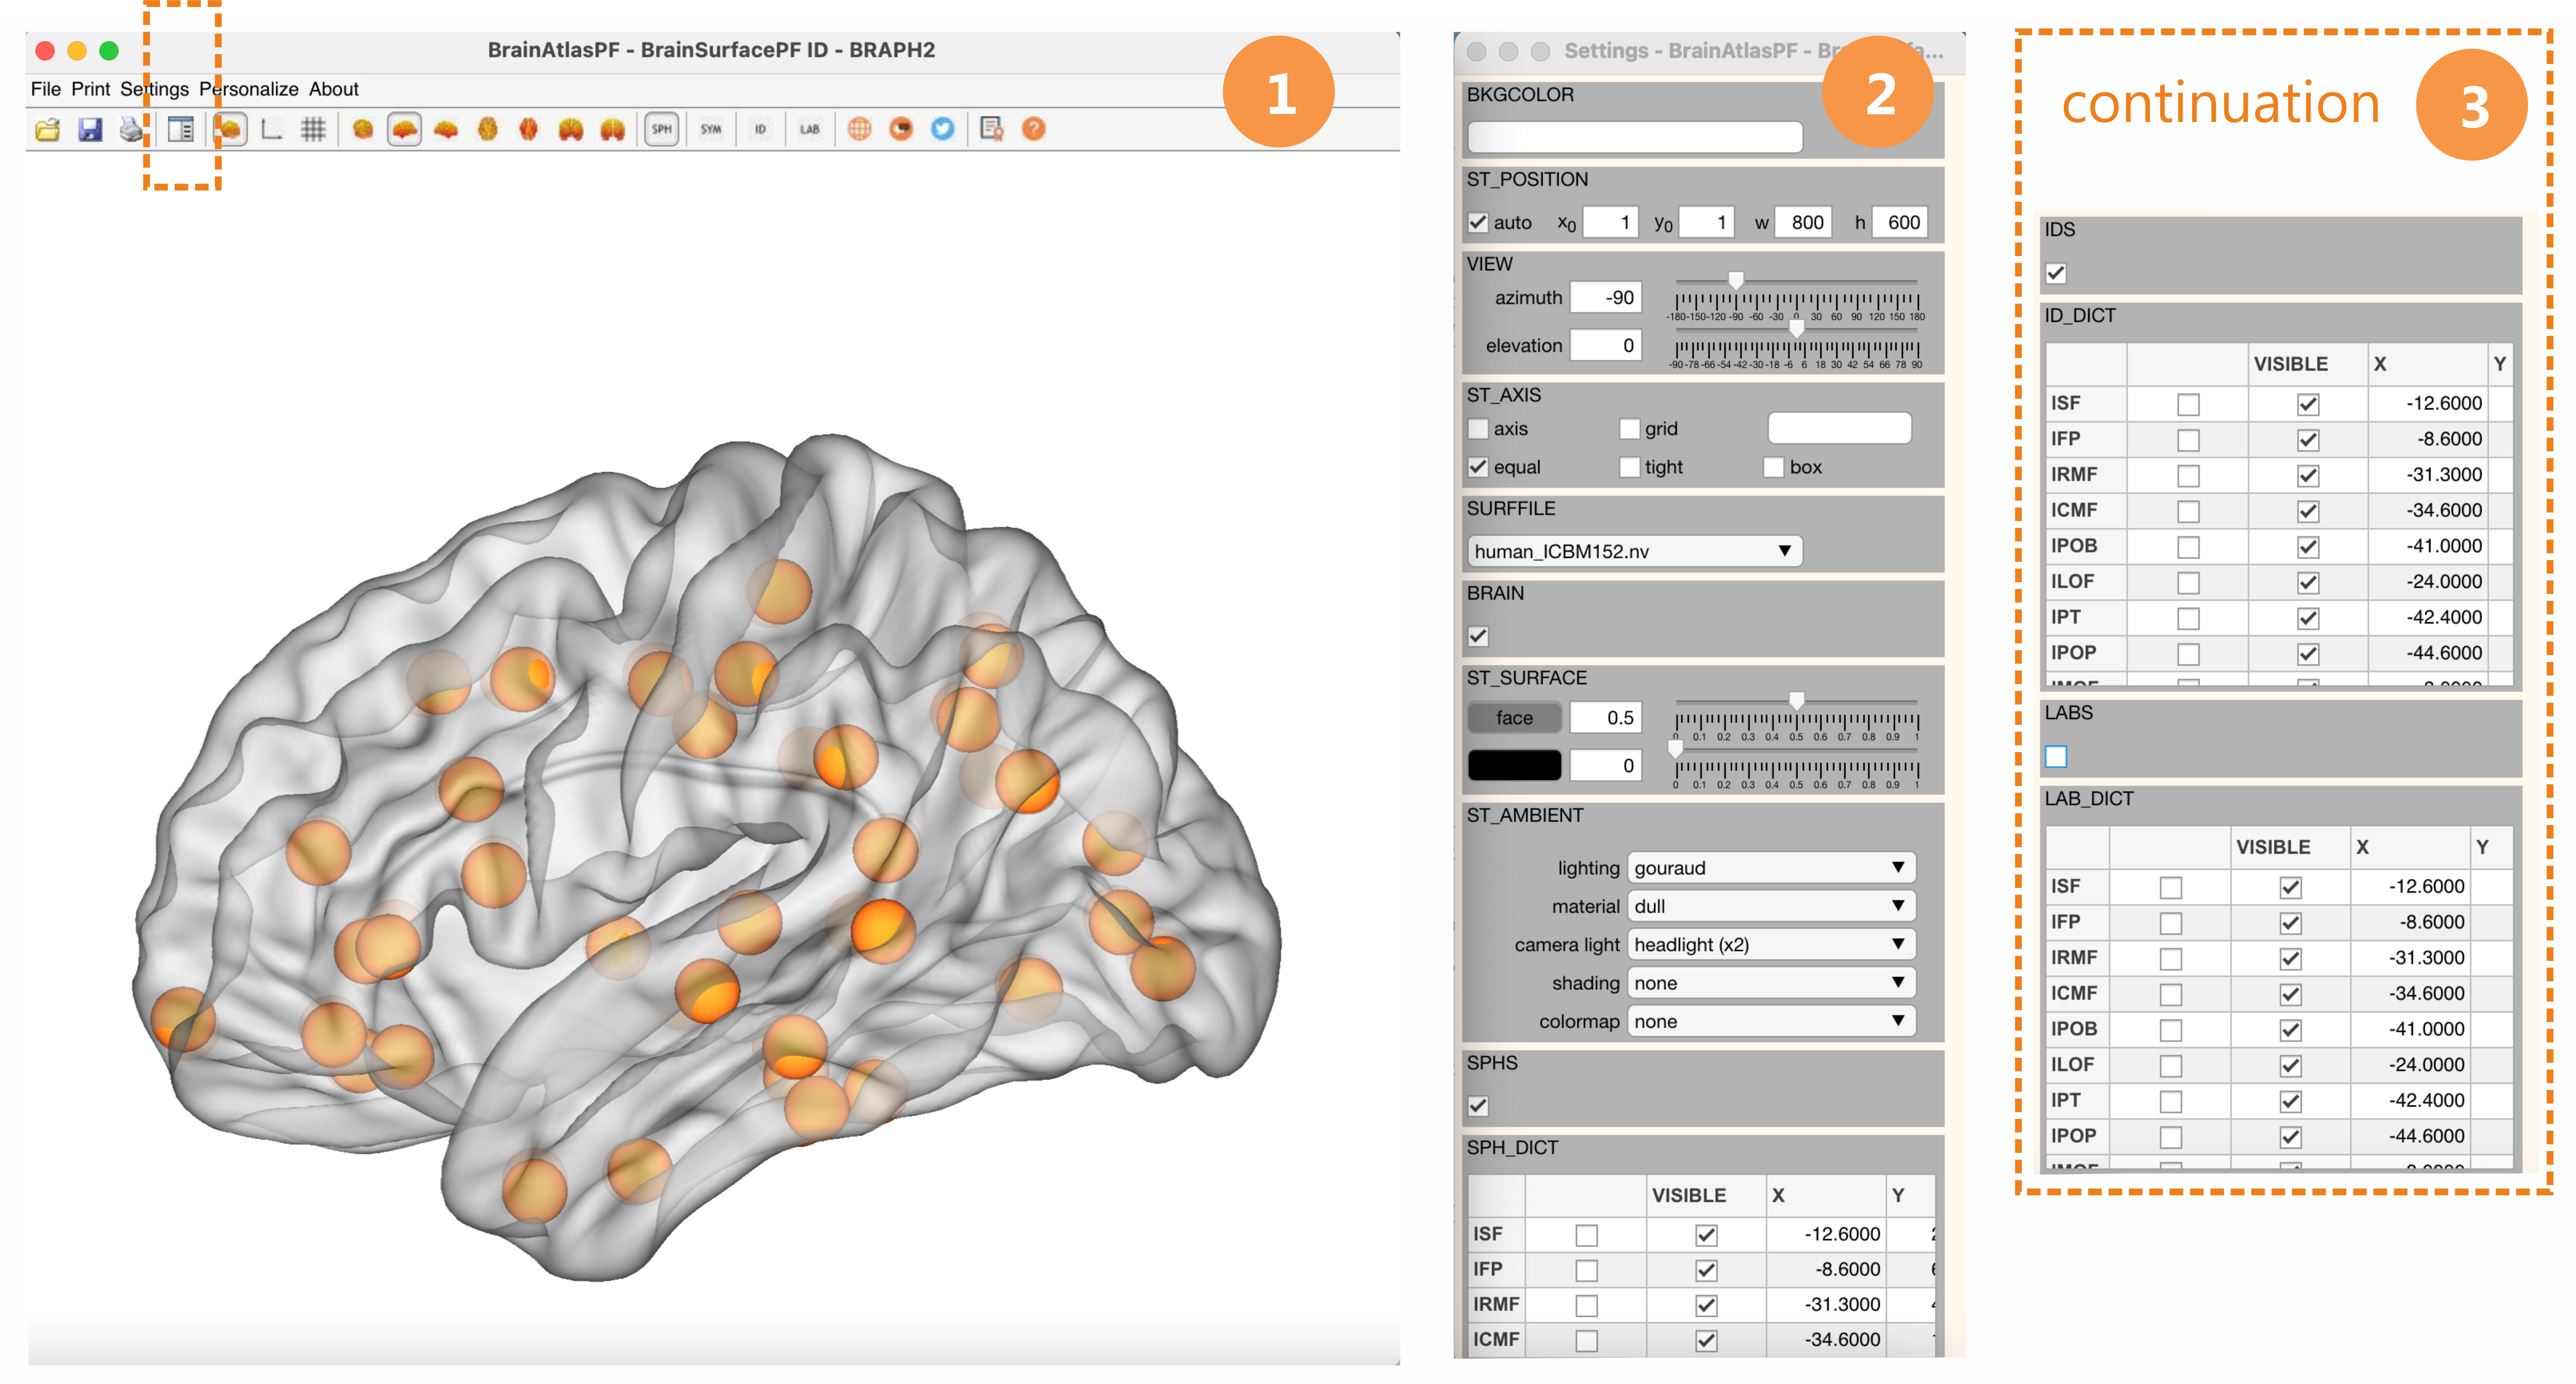
\includegraphics[height=10cm]{tut_ba/fig6.png}}
	{Brain Atlas GUI.}
	{
	Changing the visualization of the brain atlas. 
	}

This window allows you to change different options, which are important to create a final figure with all the nodes included in your analysis, which is often included within the 1st figure of a manuscript.

Most things in this panel are intuitive and again we suggest that you try different options until you achieve the visualization you want.
Some things that might not be intuitive is the difference between spheres and symbols (the first one is the geometrical structure of a node, whereas the second is just a dot inside the sphere that denotes the presence of a region). 

If you wish to change the size of the spheres of all nodes, you need to right click and select other nodes in the first column, change the size of one node and right click to select "apply to selection".

The same applies if you want to change the colour of all nodes in the FACECOLOR column. Here the colors correspond to the hexadecimal form of RGB colors, which can be found online.

There are many possibilities for visualization. Here is just one example:

\fig{figure*}
	{fig:08}
	{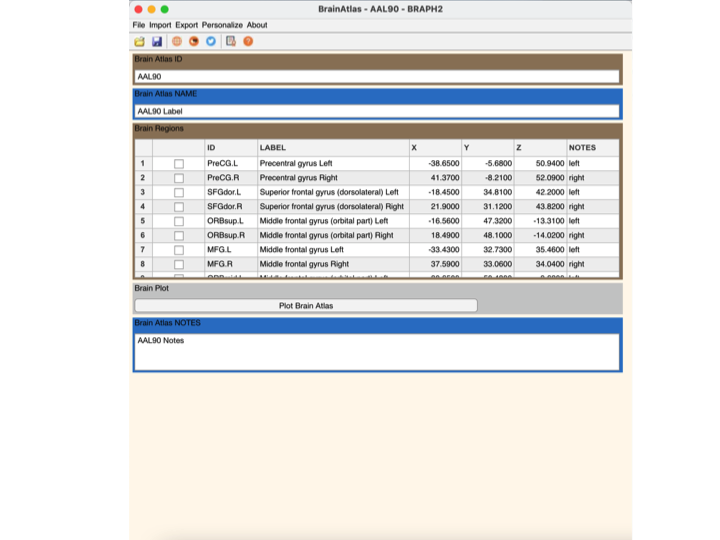
\includegraphics[height=10cm]{tut_ba/fig8.png}}
	{Brain Atlas GUI.}
	{
	One example of a visualization of the brain atlas. 
	}

\clearpage
\section{Export the Figure}

To export and save a figure, you can select print from the brain atlas GUI and select one of the various options we provide \Figref{fig9}.

\fig{figure*}
	{fig:09}
	{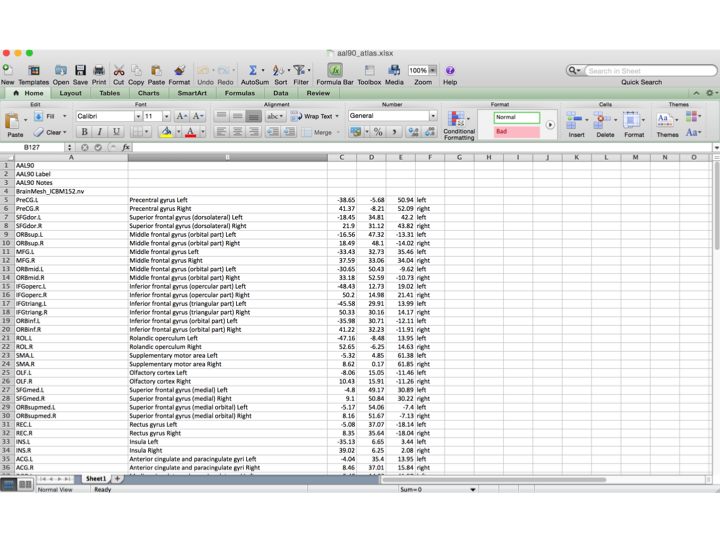
\includegraphics[height=10cm]{tut_ba/fig9.png}}
	{Brain Atlas GUI.}
	{
	How to save a figure in BRAPH 2.0. 
	}

\end{document}